\chapter{ESTUDO DE CASO}
\thispagestyle{empty}

Este capítulo apresenta um estudo de caso do CloudOoo e sua implantação num ambiente dedicado.

Para este estudo foram escolhidas duas formas de instalação: a primeira a partir do uso do SlapOS, subseção \ref{slapos}; a segunda a partir do uso direto do \textit{buildout}, forma que é principalmente utilizada para desenvolvimento e para serviços do NSI.

Não existe praticamente diferença entre ambas as instalações, exceto pelo tempo que levam, e configuração final.

Além disso este capítulo também apresentará uma avaliação quanto a forma de desenvolvimento do CloudOoo em comparação a sua versão anterior e do uso de técnicas ágeis.


\section{Aplicações relacionadas ao CloudOoo}

Com seus quase três anos de produzido o CloudOoo já vem sendo utilizado a muito por três principais aplicações, sendo uma delas diretamente responsável por sua instalação, como citado na seção \ref{insslapos} .

A subseções a seguir apresentam sobre essas aplicações.


\subsection{Biblioteca Digital}

A Biblioteca Digital da Rede Nacional de Pesquisa e Inovação (RENAPI), é um projeto que visa disponibilizar um acervo bibliográfico digital para contribuir com a disseminação de material científico e tecnológico produzido na rede de Educação Profissional Científica e Tecnológica (EPCT), sendo esse material periódicos, teses, monografias, artigos entre outros. Assim esse disseminação visa colaborar na qualificação do material humano digitalizado e na disseminação de conhecimento.

Este projeto é um dos principais desenvolvidos no Núcleo de Pesquisa em Sistemas de Informação (NSI), que conta atualmente com 20 bolsistas e 20 pesquisadores.


\subsection{ERP5}

Um ERP é capaz de integrar processos e dados de uma organização, através de recursos tecnológicos que padronizam e automatizam os mesmos.

Muito embora seja um sistema propriamente dito, ele foca mais em processos do que em funcionalidades, ele mascará informações em funcionalidades transparentes \cite{PITRE-DESAI}.

No entanto, apesar de trazer muitas vantagens a organização, esse processo de automatização, de forma geral, é longo, de alto custo e complexidade, e até mesmo difícil de implementar.

De acordo com \citeonline{SMETS-CARVALHO}, esta situação que motivou a criação do ERP5, cujas ferramentas são de código aberto, permitindo que a organização modifique-o a fim de torná-lo mais flexível aos seus processos.

Ele também incorpora conceitos avançados como o de banco de dados orientados a objetos, um sistema de gerenciamento, de sincronização, variação, \textit{workflows}, e possibilita a implementação de \textit{Business Templates}.

Compreende-se assim o ERP5, como sendo um ERP de baixo custo de implantação e alta tecnologia para pequenas e médias empresas.


\subsection{SlapOS}
\label{slapos}

O SlapOS é um sistema operacional de código aberto para o uso de redes distribuídas em computação em nuvem, que se baseia em que tudo se trata de processos.

Para \citeonline{SMETS-CERIN-COURTEAUD} a computação em nuvem é dividida em três camadas, infraestrutura como serviço (IaaS), Plataforma como Serviço (PaaS) e \textit{Software} como Serviço (SaaS). Na IaaS esta o funcionamento virtual do computador e seu armazenamento, sob o ele é construído o Paas, que funciona como coração dos serviços, como servidor e bancos de dados. Finalmente sobre Paas estão as aplicações de uso do usuário.

Através de uma API unificada e simples, que requer poucos minutos para aprendizagem, este sistema combina computação em grade e o conceito de ERP para fornecer estas categorias previstas na compução em nuvem.

Dada sua abordagem unificada e arquitetura modular, ele tem sido usado como uma ferramenta de testes para \textit{benchmark} de bancos de dados NoSQL e para otimização do processo de alocação em nuvem.


\section{Ambiente de desenvolvimento}
\label{computadores}

O estudo apresentado neste trabalho foi desenvolvido no NSI e contou com a disponibilidade de um computador com processador Intel Core I5 CPU 650 3.20 x4, 4GB de memória RAM, 320GB de HD; bem como de um notebook com processador Intel Core 2 Duo CPU 2.13 Hz, 8GB de memória 50GB de HD disponíveis para o sistema; além de dois servidores do NSI um de processador Xeon CPU E5335 2.00 x8, 14 GB de memória e 20GB de HD e um segundo com processador Xeon CPU E5335 2.00 x4, 4GB de memória e 20GB de HD, em uma máquina virtual.

Os dois primeiros computadores contavam com o sistema operacional Ubuntu 12.04 Lt, enquanto os servidores utilizavam o sistema operacional Debian 6.0.


\section{Processo de Desenvolvimento}

Para \citeonline{PRESSMAN}, a garantia da qualidade de software esta diretamente ligada ao emprego de testes sobre o mesmo, onde esses testes representam a expectativa do usuário sobre a aplicação, e podem ser empregados de forma automatizada ou manual. Embora testes automatizados tendam a gastar mais tempo em relação a programação dos mesmos, sua cobertura sobre o produto garante menor porcentagem de erros quando executada a aplicação.

A técnica TDD (\textit{Test-Driven Development}), ou desenvolvimento orientado a testes, defende o desenvolvimento dos testes antes do desenvolvimento da parte funcional da aplicação, dado que os testes também fazem parte da mesma. A eficácia dela garanti que todas as expectativas da aplicação sejam testadas e portanto garantidas ao usuário.

No inicio da parceria do NSI e Nexedi no desenvolvimento do CloudOoo quase não se utilizavam testes, entretanto com seu crescimento como produto e apresentada a dificuldade em mantê-lo estável foi dado o começo ao desenvolvimento de teste, a técnica TDD ainda não era empregada neste primeiro momento em função da porcentagem ja desenvolvida do produto, atualmente porém vêm sendo empregada diretamente.

Segundo \citeonline{ASTELS}, projetos que utilizam TDD devem possuir uma suíte exaustiva de testes que por sua vez determinam o código que deve ser escrito. No entanto para uma aplicação de serviço web, existe certo grau de dificuldade de começar do zero apenas com testes, tendo por justificativa suas dependências como outras aplicações bem como a utilização de rede por este. 

Para a realização de testes unitários no CloudOoo foi preciso antes o desenvolvimento de \textit{scripts} que pudessem interligar todas as bibliotecas envolvidas para o funcionamento do mesmo. Também foram desenvolvido \textit{scripts} que ``ligam'' a aplicação e realizam testes na rede local, a fim de garantir que as respostas estejam corretas quando este serviço estive ativo e responder a conexões distantes.

Além dos testes, outra ferramenta que garante o desenvolvimento do CloudOoo é o uso de um sistema de controle de versão, como o \textit{subversion}, que era utilizado na versão 2.0, e que atualmente foi trocado pelo \textit{git} em função de vantagens como, por exemplo, o controle de versões distribuído. A importância desta ferramenta esta no controle do crescimento da aplicação, que por momentos contou com uma equipe de desenvolvimento sem contato constante e em diferentes períodos.

Assim por meio de ferramentas que podiam acompanhar as modificações da aplicação, bem como reverter determinadas alterações em casos de erros posteriores na mesma e dar um detalhamento de quando essas modificações ocorreram, foi possível seguir com este desenvolvimento.

Sob certo ponto de vista o uso destas práticas sugere sobre o desenvolvimento do CloudOoo severas semelhanças com os métodos ágeis, muito embora não exista a definição propriamente dita de nenhuma delas aplicadas diretamente sobre o projeto.

Em seu artigo \citeonline{SILVA-MONNERAT-CARVALHO}, comprovam o uso do TDD no CloudOoo, e de suas complicações de emprego, uma vez que inicialmente não existia total proficiência por parte dos desenvolvedores. Além disso foi verificado sobre o estabilidade do desenvolvimento do projeto, tomando por base a lista de mudanças armazenadas pelo controle de versão. Observou-se através deste artigo que embora no incio do projeto nenhum teste falhasse, conforme o mesmo foi acrescido de mudanças e novas funcionalidades testes que antes passavam passaram a apresentar erros antes não conhecidos, precisando assim de correções.

Estas implicações trazem ao meio de software uma compreensão muito similar ao do ramo de indústria, no que se desrespeita a aplicação de novas técnicas para garantir que quando um produto chega ao meio de produção possa continuar estável ao uso.


\section{Processo de instalação}

Para instalação via SlapOS, foi definido como pré-requisito a instalação do próprio SlapOS, sendo este dependente apenas da existência da instalação do Python, em qualquer versão uma vez que o SlapOS instala todos seus requisitos de funcionamento, inclusive o próprio Python. Variando de acordo com o sistema escolhido podem ser necessários demais pacotes de dependências de sistema.

Da mesma forma, para instalação via \textit{buildout}, forma um pouco mais simples, é necessário igualmente possuir a instalação do  Python e do Git como pré requisitos, uma vez que através deles e do uso da biblioteca \textit{bootstrap}, disponível em \cite{BOOTSTRAP}, é possível gerar o \textit{script bin/buildout}, bem como utilizá-lo para viabilizar a instalação do CloudOoo por seus arquivos de configuração, ou receitas.

Nas próximas subseções serão apresentadas as devidas instalações.


\subsection{Instalação via SlapOS}

Esta instalação foi realizada a partir da modificação do tutorial de instalação do ERP5 no SlapOS \cite{ERP5-SLAPOS}, o qual passa por modificações ocasionalmente em função das atualizações frequentes desta ferramenta.

Nestas subseções será apresentado o tutorial já modificado em sequência de instalação:


\subsubsection{Instalação do SlapOS}
\label{insslapos}

Está primeira subseção é a instalação padrão para qualquer ferramenta que utilize o SlapOS.

É aconselhado que seja realizada a instalação na pasta raiz do sistema, assim requerendo privilégios para instalação. É possível para o usuário optar por instalá-lo em sua pasta de usuário com algumas modificações no tutorial, entretanto em determinados momentos será podem ocorrer erros inesperados, e a exigência do uso de privilégio de qualquer forma.

Como é possível notar no código \ref{slapos-1}, cria-se uma pasta para instalação em \textit{/opt/slapos}, e também um arquivo de configuração \textit{buildout}.

Após a criação deste arquivo, através do uso do Python, é realizada a execução de um \textit{bootstrap} próprio da Nexedi.

{\singlespace
\begin{lstlisting}[caption=Primeira parte da instalação do SlapOS,language=bash,label={slapos-1}]
$ sudo mkdir /opt/slapos 

$ cd /opt/slapos
$ touch buildout.cfg
$ vi buildout.cfg

[buildout]
extends =
  http://git.erp5.org/gitweb/slapos.git/blob_plain/refs/tags/slapos-0.57:/component/slapos/buildout.cfg

$ sudo python -S -c 'import urllib2; print urllib2.urlopen("http://www.nexedi.org/static/\
packages/source/slapos.buildout/bootstrap-1.5.3-dev-SlapOS-002.py").read()' | python -S -

$ sudo bin/buildout -v
\end{lstlisting}
}

Com o termino do \textit{bootstrap} é executado o \textit{script bin/buildout}, que realiza a instalação dos componentes necessários ao SlapOS.


Após a instalação dos componentes e dependências é preciso configurar o mesmo, no código \ref{slapos-2}, existe um exemplo de arquivo de configuração e logo em seguida na figura \ref{slapos-rede}, existe a configuração de rede para uso do SlapOS.

É necessário que o \textit{slapproxy} seja iniciado e mantido rodando em \textit{background} sempre que esta máquina estiver ligada e/ou em uso, ele representa funcionalidades de conectividade do SlapOS \textit{master}.

{\singlespace
\begin{lstlisting}[caption=Arquivo de configuração do SlapOS,language=python,label={slapos-2}]
$ touch slapos.cfg

[slapos]
software_root = /opt/slapgrid
instance_root = /srv/slapgrid
master_url = http://127.0.0.1:5000/
computer_id = vifibnode

[slapformat]
computer_xml = /opt/slapos/slapos.xml
log_file = /opt/slapos/slapformat.log
partition_amount = 5
bridge_name = br1331
partition_base_name = slappart
user_base_name = slapuser
tap_base_name = slaptap
ipv4_local_network = 10.0.0.0/16

[slapproxy]
host = 127.0.0.1
port = 5000
database_uri = /opt/slapos/proxy.db

\end{lstlisting}
}

{\singlespace
\begin{lstlisting}[caption=Configurações de rede do SlapOS,language=sh,label={slapos-rede}]
$ sudo bin/slapproxy -vc /opt/slapos/slapos.cfg
$ sudo brctl addbr br1331
$ sudo ip l s dev br1331 up
$ sudo ip a l dev br1331 fd00::1/64
$ sudo vi /etc/network/interfaces

  auto br1331
  iface br1331 inet6 static
    adress fd00::1
    netmask 64
    bridge_ports none

$ sudo bin/slapformat -c /opt/slapos/slapos.cfg
$ sudo bin/slapgrid -c /opt/slapos/slapos.cfg

\end{lstlisting}
}

É possível reparar que o SlapOS é uma ferramenta adaptada ao IPV6, e necessariamente é preciso configurá-lo através da interface \textit{br1331}.

O \textit{script /etc/network/interfaces} do sistema também é configurado para habilitar as funcionalidades de IPV6, a fim de que não seja preciso iniciá-las sempre que reinicie o sistema.

Por fim nas duas ultimas linhas do código \ref{slapos-rede} são executados os \textit{scripts slapformat}  e \textit{slapgrid}, eles são responsáveis por registrar seu computador na nuvem e seus devidos \textit{slots} além de habilitar o cliente SlapOS em seu computador, respectivamente.


\subsubsection{Instalação do CloudOoo}

Após realizada a instalação do SlapOS, o passo de instalação de ferramentas através do mesmo é consideravelmente simples.

Para requerer a instalação do CloudOoo é necessário utilizar o \textit{slapconsole} citando o arquivo de configuração citado na subseção \ref{insslapos}, assim com o uso de uma instância do SlapOS(\textit{slap}), referenciada na terceira linha da figura \ref{requisicao-software}, informa-se a esta instância qual será sua função, isto é, seu produto específico. 

A partir do uso do \textit{slapgrid} a parte referente aos componentes deste produto será instalado de forma compilada pelo \textit{Buildout}.


{\singlespace
\begin{lstlisting}[caption=Requisição de instalação do CloudOoo no SlapOS,language=bash,label={requisicao-software}]
$ bin/slapconsole /opt/slapos/slapos.cfg

import slapos.slap.slap
slap = slapos.slap.slap()
slap.initializeConnection('http://127.0.0.1:5000/')

slap.registerSupply.supply(
    "http://git.rp5.org/gitweb/slapos.git/blob_plain/cloudooo:/software/cloudooo/software.cfg",
    computer_guid="vifibnode")
#teste que retorna id da instancia
computer_particion.getId()

$ sudo bin/slapgrid-sr -c /opt/slapos/slapos.cfg

\end{lstlisting}
}

Nesta referência em particular o ponteiro esta voltado para o \textit{branch} do CloudOoo, em função de suas configurações próprias que não foram incorporadas ao projeto do SlapOS.

Após a instalação dos componentes é necessário requerer uma instância, como em \ref{requisicao-instancia}.

Este processo também requer o uso do \textit{slapconsole}, de forma semelhante a instalação de componentes, no entanto é necessário fornecer um título a sua instância e é possível verificar se a mesma foi criada requirindo, por exemplo, seu \textit{id}.

{\singlespace
\begin{lstlisting}[caption=Requisição de uma instância do CloudOoo via SlapOS,language=bash,label={requisicao-instancia}]
$ bin/slapconsole /opt/slapos/slapos.cfg

import slapos.slap.slap
slap = slapos.slap.slap()
slap.initializeConnection('http://127.0.0.1:5000/')

computer_particion = slap.registerOpenOrder(
    "http://git.rp5.org/gitweb/slapos.git/blob_plain/cloudooo:/software/cloudooo/software.cfg",
    "Meu CloudOoo")
#teste que retorna id da instancia
computer_particion.getId()

$ sudo bin/slapgrid-cp -c /opt/slapos/slapos.cfg

\end{lstlisting}
}

Por fim é utilizado novamente o \textit{slapgrid}, mas desta vez com novos parâmetros para que a criação da instância seja finalizada.

Por se tratar de um serviço web em um sistema de nuvens, esta instalação compreende que após terminada deverá iniciar um servidor do CloudOoo pelas configurações estabelecidas no software.


\subsection{Instalação do CloudOoo.git}
\label{clougit}

Esta segunda instalação foi criada para ser mais flexível aos projetos do NSI que também utilizam o CloudOoo, bem como aos que tenham intenção de colaborar com esta ferramenta. 

Esta instalação esta disponível no Github do NSI, \cite{BUILD-CLOUDOOO}, e possui um \textit{README} com instruções para instalação. 

Além disso esta instalação esta orientada a fazer download do repositório igualmente disponível no Github do NSI, em \cite{NSI-CLOUDOOO}, que se mantém sempre na última versão de desenvolvimento, a mais atual.

Após o download do \cite{BUILD-CLOUDOOO}, são necessárias apenas duas instruções para esta instalação, \ref{buildout-cloudooo}:

{\singlespace
\begin{lstlisting}[caption=Modo de instalação do cloudOoo \cite{BUILD-CLOUDOOO},language=bash,label={buildout-cloudooo}]

$ python -S -c 'import urllib2; exec urllib2.urlopen("http://python-distribute.org/boostrap.py").read()'

$ bin/buildout -vv

\end{lstlisting}
}

Na primeira etapa utiliza-se o Python para fazer \textit{download} e rodar o \textit{script} do \textit{boostrap}, este irá fazer o download e disponibilizar o \textit{Buildout}. 

Ao termino desta fase, com o \textit{script buildout} acrescido de argumentos no intuito de torná-lo verboso e do arquivo padrão de configuração (\textit{buildout.cfg}), ocorre a instalação do CloudOoo e todos os componentes necessários, entre eles o LibreOffice, FFMPEG, ImageMagick e demais.

Diferentemente da instalação via SlapOS o servidor do CloudOoo não fica disponível automaticamente para uso, é preciso ainda utilizar o \textit{script bin/supervisord} para dar inicio ao servidor.

Ainda caso o usuário desejar é possível trocar a porta de funcionamento do servidor no arquivo \textit{cloudooo.cfg}, bem como outras configurações padrão, como o limite do uso de memória.


\section{Processos de requisições}

Para estabelecer conexão entre um cliente qualquer e o CloudOoo é necessário o uso de uma biblioteca compatível ao XMLRPC. No código \ref{conexao} foi realizado um exemplo de cada requisição básica disponível para todos \textit{handlers}, através de uma conexão estabelecida pela biblioteca \textit{xmlrpclib}:

{\singlespace
\begin{lstlisting}[caption=Exemplo prático de uso do CloudOoo,language=python,label={conexao}]
from base64 import encodestring
from xmlrpclib import Server

conexao = Server("http://localhost:23000")

arquivo = open("test.ogv").read()

novo-arquivo = conexao.convertFile(encodestring(arquivo), 'ogv', 'mpeg')

info = conexao.getFileMetadataItemList(encodestring(arquivo), 'ogv')

nova-info = conexao.updateFileMetadata(encodestring(arquivo), 'ogv', dict(Titulo="Arquivo teste"))

\end{lstlisting}
}

Na linha 6 do código a variável \textit{arquivo} recebe o conteúdo do arquivo \textit{test.ogv}.

Para conversão deste, na linha 8, é preciso codificá-lo para que durante sua passagem do cliente para o servidor esse arquivo não seja danificado, esta codificação realizada pelo uso da biblioteca \textit{base64}.

No momento da conversão o servidor vai receber os dados do cliente, vai decodificar o arquivo e identificá-lo como um arquivo de vídeo, sendo assim o mesmo será encaminhado para o FFMPEGHandler, que por sua vez irá convertê-lo para o formato \textit{mpeg}.

O FFMPEGHandler também será o responsável pelos métodos de \textit{getFileMetadataItemList}, linha 10, e \textit{updateFileMetadata}, linha 12, nos quais serão realizados respectivamente a extração e inserção de metadados no arquivo.

Na linha 12 é possível notar que para inserção de metadados, os novos dados a serem passados devem estar em um dicionário.

Observe também que nesta inserção de metadados, foi utilizado o \textit{nova-info}, como resposta da requisição de inserção de metadados. Isto porque esta requisição do CloudOoo retorna um arquivo com os dados inseridos no mesmo, e que já se encontra codificado para transporte.

Além destas requisições comuns a todos os \textit{handlers} existem também requisições que foram previamente implantadas apenas para documentos:

\begin{itemize}
    \item{getAllowedExtensionList: retorna extensões permitidas para determinado arquivo;}
    \item{getChapterItem: retorna o capítulo selecionado do documento;}
    \item{getChapterItemList: retorna todos capítulos do documento;}
    \item{getColumnItemList: retorna colunas da tabela selecionada;}
    \item{getImage: retorna imagem selecionada;}
    \item{getImageItemList: retorna lista de imagens em documento;}
    \item{getLineItemList: retorna lista de linhas da tabela selecionada;}
    \item{getParagraph: retorna parágrafos selecionado;}
    \item{getParagraphItemList: retorna lista de parágrafos de um documento;}
    \item{getTable: retorna tabela selecionada;}
    \item{getTableItemList: retorna lista de tabelas no documento;}
    \item{system.listMethod: retorna lista de métodos disponíveis no servidor.}
\end{itemize}

\section{Uso do CloudOoo na Biblioteca Digital}

Para disponibilizar seu acervo, a Biblioteca Digital tem como regra converter os arquivos recebidos seu formato livre compatível, para isso utiliza de requisições ao CloudOoo. Na figura \ref{submeter}, existe um exemplo de submissão de arquivos, do tipo Relatório, o qual passará pela conversão de DOC para ODT através de uma requisição ao CloudOoo, após a aprovação \ref{aprovar}:

\begin{figure}[ht]
    \centering
    \scalebox{0.4}{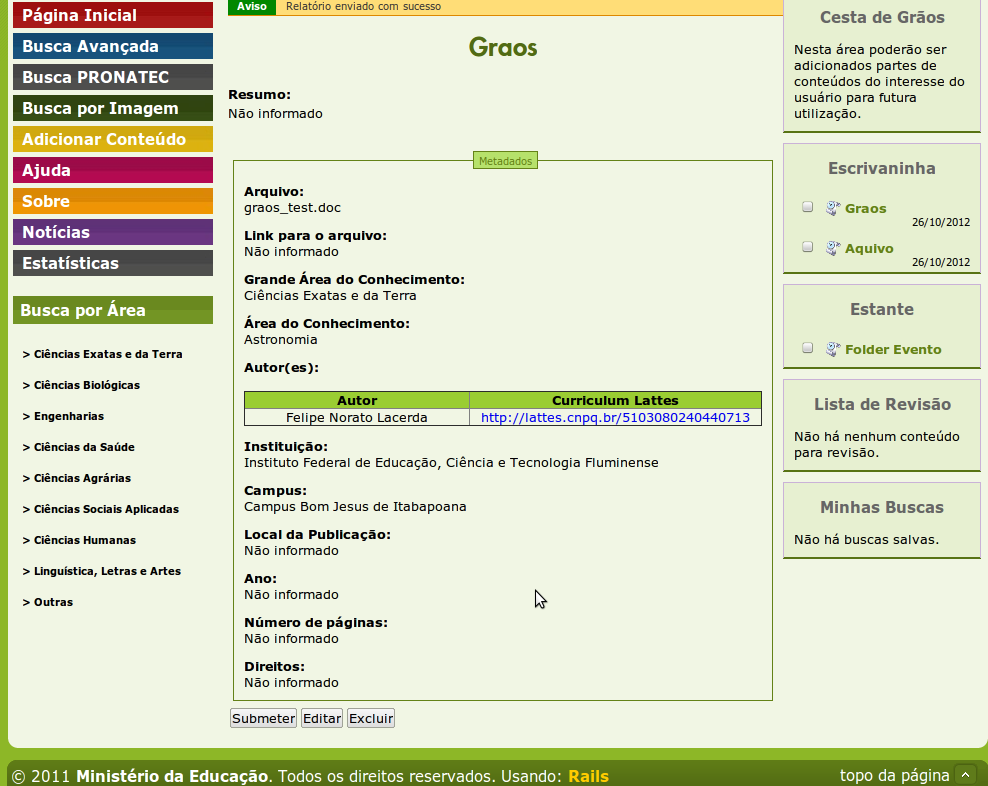
\includegraphics{figuras/submeter}}
    \caption{Pagina de submissão de documentos da Biblioteca Digital}
    \label{submeter}
\end{figure}

\begin{figure}[ht]
    \centering
    \scalebox{0.4}{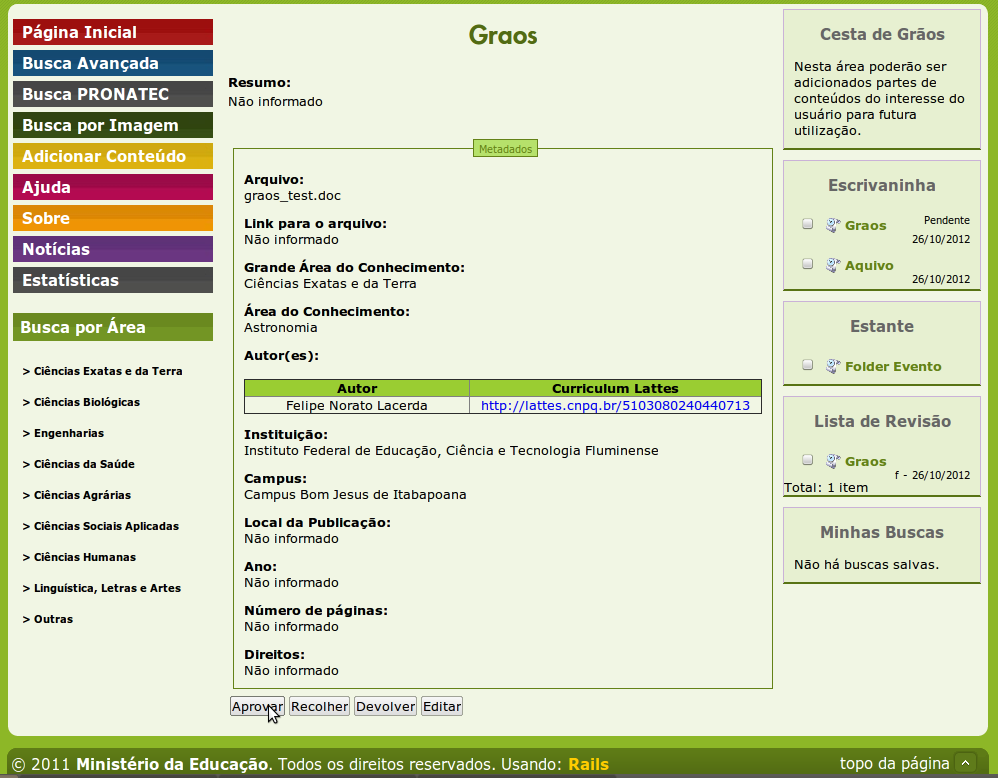
\includegraphics{figuras/aprovar}}
    \caption{Pagina de aprovação de documentos da Biblioteca Digital}
    \label{aprovar}
\end{figure}

\newpage
Nas figuras não é implícito o uso da ferramenta, entretanto, uma vez que essa funcionalidade requer o uso de documentos em formato livre para realização de suas tarefas, é requerido o uso do CloudOoo para converter o arquivo em questão para um padrão livre e posteriormente realizar a funcionalidade de ``granularização''.

\begin{figure}[ht]
    \centering
    \scalebox{0.4}{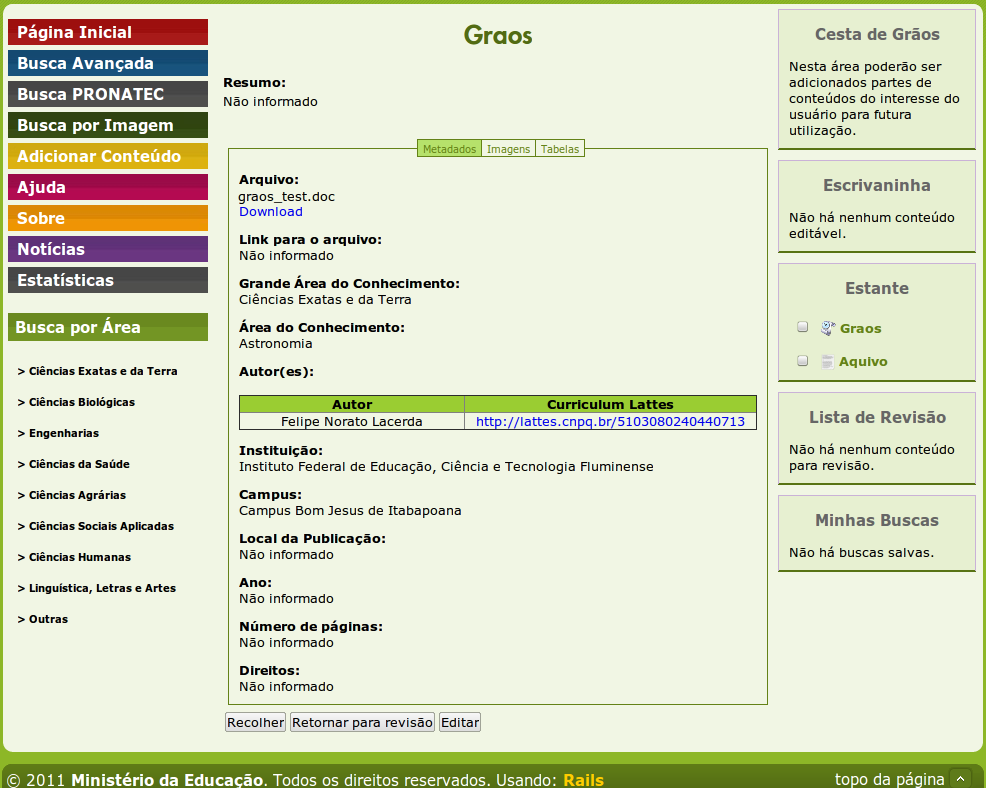
\includegraphics{figuras/metadados}}
    \caption{Pagina de exibição de metadados de documentos da Biblioteca Digital}
    \label{metadados}
\end{figure}

\newpage
Na figura \ref{metadados} há uma demonstração da funcionalidade de extração de metadados, enquanto os grãos encontram-se nas figuras \ref{imagens}:

\begin{figure}[ht]
    \centering
    \scalebox{0.4}{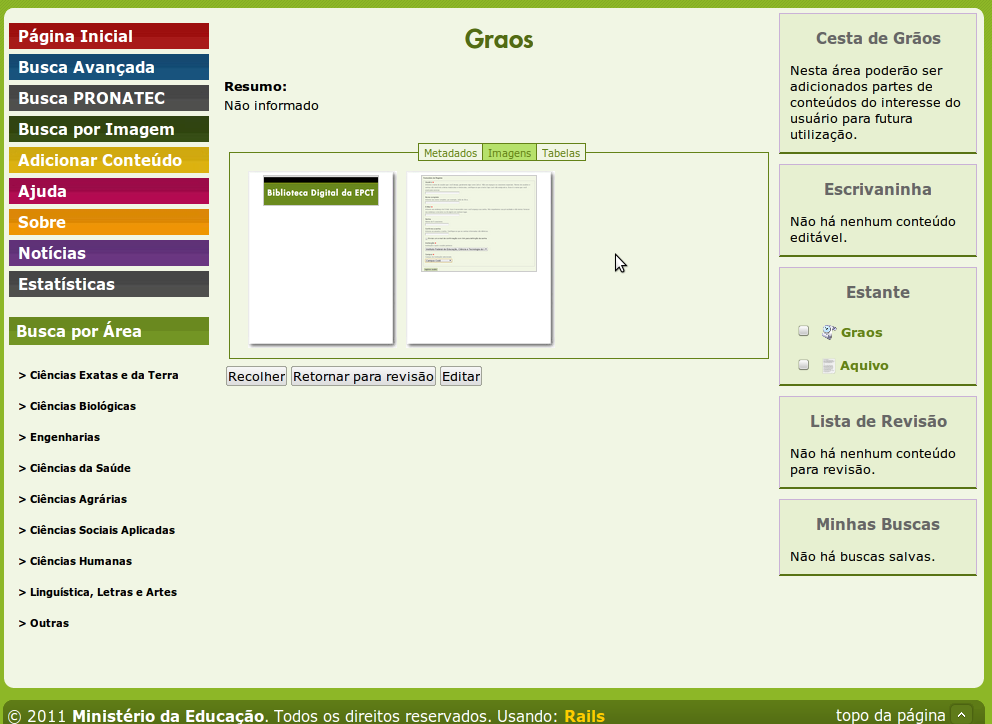
\includegraphics{figuras/imagens}}
    \caption{Pagina de exibição de grãos do tipo imagem de documentos da Biblioteca Digital}
    \label{imagens}
\end{figure}

\newpage
Os grãos extraídos pelo processo de ``granularização'' são separados em imagens(\ref{imagens}) e tabelas, que não existem nesse caso, e dispostos para visualização do usuário.


\newpage
\section{Performance}

Para estabelecer diferença de performance em relação as versões anteriores do CloudOoo foram considerados dois testes.

O primeiro deles realizado em um trabalho anterior, por \citeonline{MONNERAT}, contava 3699 documentos no formato ODT que foram selecionados previamente, entre eles alguns documentos inválidos e outros em formatos desconhecidos. Por ser a conversão mais utilizada, foi decido que neste teste estes documentos seriam convertidos para PDF. 
Este teste foi realizado por meio do uso de um \textit{script}, neles além de prover a conversão também era provido o armazenamento do tempo de cada conversão, bem como o tempo total que todas as conversões levaram em cada versão do CloudOoo.

No resultado do primeiro teste notou-se que o OOOD 2.0 levará mais tempo para realizar a conversão de cada documento,entretanto por ser mais estável levou 10 horas para realizar o teste e apresentou 12 erros, enquanto o OOOD 1.0 apresentou 531 erros e levou 11 horas para realizar o teste.

No segundo teste foram escolhidos arquivos distintos, representado no código \ref{carga}, este teste selecionou 3 diferentes documentos DOC para serem convertidos para ODT; 3 documentos com PDF para serem convertidos para TXT, 1 arquivo de vídeo AVI de aproximadamente 100 MB que seria convertido para THEORA; um arquivo de áudio MP3 de aproximadamente 3 MB para ser convertido para VORBIS; e por fim uma imagem PNG de aproximadamente 30 KB para ser convertida para JPG.

\newpage
{\singlespace
\begin{lstlisting}[caption=\textit{Script} de teste,language=python,label=carga]
from random import randint
from base64 import encodestring, decodestring
from datetime import datetime
from xmlrpclib import ServerProxy
import magic


mime_decoder = magic.Magic(mime=True)

documents = ['ISSCWR6PaperTemplate.doc','SiteLeaderAppWinter2012.doc', 'Estonia.doc']
pdfs = ['Bankruptcies.pdf', 'WIA-IM_tfw_studentguide.pdf', '2012FinancialRpt.pdf']

type_convert_choices = { 0: [documents, "doc", "odt", 'application/vnd.oasis.opendocument.text'],
                  1: ["test.png", "png", "jpg", 'image/jpeg'],
                  2: ["test.mp3", "mp3", "ogg", 'application/ogg'],
                  3: ["test.avi", "avi", "ogv", 'application/ogg'],
                  4: [pdfs, "pdf", "txt", 'text/plain']
                }


proxy = ServerProxy("http://localhost:23000/RPC2")
id = 0
process = []

while True:

  name = 'test'
  file, source_format, destination_format, mime = type_convert_choices[randint(0,4)]
  data = ''
  if type(file) == str: 
    data = open(file).read()
  else:
    name =file[randint(0,2)]
    data =  open(name).read()
  done, mimetype = False, False
  try:
    file = proxy.convertFile(encodestring(data), source_format, destination_format)
    mimetype = mime_decoder.from_buffer(decodestring(file))
    if mimetype == mime:
      done = True
  except:
    done = "Error"
  process.append([id, name, source_format, mime, destination_format, mimetype, done, '\n'])
  id += 1

content = "  id     |          file       |     source         |   dest            |    done          \n" + str(process)
log = open('log.txt', 'w')
log.write(content)
log.close()

\end{lstlisting}
}

O objetivo deste segundo teste era focar nas conversões de arquivos para formatos abertos, que são mais utilizados nos projetos que o CloudOoo atende. 

Além disso a perspectiva era que um menor número de erros aparecesse em função dos inúmeros tratamento utilizados nesta ferramenta. Também haveria um menor número de conversões que a versão anterior em função do tamanho e tempo que arquivos de vídeo, imagem e áudio consomem comparados a documentos.

Para saber se as conversões foram realizadas com sucesso eram verificados os \textit{mimetypes} de cada conversão de acordo com o esperado.

Infelizmente não foi possível a utilização de diversos arquivos aleatoriamente como seria o caso de um ambiente de produção, em função da dificuldade para adquirir estes arquivos por meio da internet que tem sido cada vez mais restrita a downloads.

Neste segundo teste foram utilizados dois computadores diferentes de desenvolvimento, citados em \ref{computadores}, no notebook e no servidor de 4GB de memória.

No notebook a performance foi consideravelmente estável, em 10 horas o CloudOoo realizou 2034 conversões, entre elas 405 conversões foram de DOC para ODT e apenas 3 retornaram erro; 260 foram de PDF para TXT e nenhuma retornou erro; 307 foram de AVI para OGV Theora e nenhuma retornou erro; 384 foram de MP3 para OGG \textit{Vorbis}; e 678 foram de PNG para JPG sem retorno de erro.

Resultando assim em apenas 3 erros em 10 horas.

No servidor, entretanto o resultado foi menos promissor, o teste durou apenas 3 horas em função de um erro de estouro de memória no servidor, que detinha de aproximadamente 3 GB livres para o teste, mas que não se encontrava disposto apenas para o teste uma vez que estava em uso em tempo real. 

Durante essas 3 horas foram realizadas 611 conversões, entre elas 122 conversões foram de DOC para ODT e apenas 1 retornou erro; 77 foram de PDF para TXT e nenhuma retornou erro; 91 foram de AVI para OGV Theora e nenhuma retornou erro; 114 foram de MP3 para OGG Vorbis; e 207 foram de PNG para JPG sem retorno de erro.

De forma positiva o CloudOoo se manteve estável durante essas horas tanto no notebook quanto no servidor, pois mesmo com o estoura de memória no segundo, ele se manteve ativo. Entretanto com os resultados dos teste foi constatado que com as novas funcionalidades adicionadas precisam ser revisadas em função de escalabilidade e uso em tempo real a fim de que não volte a ocorrer estouros de memória entre outros possíveis erros. 

No que respeito aos erros de documentos, dada a falta de variedade, foram todos erros relativos aos documentos PDF com proteção contra conversão.

Na tabela \ref{clooo} mostrando os resultados desses testes:

\begin{table}[!t]
\caption{Comparação entre versões do CloudOoo por meio de testes.}
\label{clooo}
\begin{tabular}{|r|c|c|c|c|p{1.5cm}|p{2cm}|p{1.5cm}|}
\hline
Versões & Documentos & Imagens & Áudio & Vídeo & Total de erros & Total de Conversões & Total de horas \\
\hline
OOOD 1.0 & 3699 & 0 & 0 & 0 & 531 & 3699 & 11 \\
\hline
OOOD 2.0 & 3699 & 0 & 0 & 0 & 12 & 3699 & 10 \\
\hline
CloudOoo & 405+260 & 307 & 384 & 678 & 3 & 2034 & 10 \\
\hline
\end{tabular} 
\end{table}

